% Supplementary material for the pyCICY package.
%
% Build with:
%     make figures            # regenerate paper/figures/*.{pdf,png}
%     pdflatex supplementary_material.tex
%
% Every figure is written twice by paper/make_figures.py: a PDF, used here,
% and a PNG of the same content, used by the repository README. GitHub
% renders PNG inline in Markdown but will not render an embedded PDF.

\documentclass[7pt]{article}
\usepackage[margin=2.5cm]{geometry}
\usepackage{graphicx}
\usepackage{amsmath}
\usepackage{amssymb}
\usepackage{booktabs}
\usepackage[hidelinks]{hyperref}
\usepackage{caption}
\usepackage{hyperref}
\usepackage{orcidlink}
\usepackage{placeins}
\usepackage{wrapfig} % Required for text wrapping

\usepackage{titlesec}
% Syntax: \titlespacing*{<command>}{<left>}{<before-sep>}{<after-sep>}[<right-sep>]
\titlespacing*{\section}{0pt}{4pt}{2pt}
\titlespacing*{\subsection}{0pt}{2pt}{1pt}

\titleformat{\section}
  {\normalfont\fontsize{12pt}{14pt}\bfseries} % Change 16pt (size) and 20pt (line spacing) as needed
  {\thesection}
  {1em}
  {}

\graphicspath{{figures/}}

\newcommand{\pkg}[1]{\texttt{#1}}
\newcommand{\CY}{Calabi--Yau}
\newcommand{\PP}{\mathbb{P}}

\title{Supplementary material: figures for the \pkg{pyCICY-X} package}
\author{B.S. Hartshorn \orcidlink{0009-0004-2853-655X} \small \url{https://github.com/brentharts/CICY}}

\begin{document}
\maketitle

\begin{abstract}
This supplement reproduces and describes every figure emitted by
\pkg{paper/make\_figures.py}. The figures fall into two groups. The first
concerns the web of complete intersection \CY{} threefolds obtained by
splitting, and the consistency checks that hold it together. The second
concerns three later additions to the package --- quantized mirror curves of
local toric \CY{} geometries, knot invariants, and hyperbolic lattices ---
together with the two threads that connect them, namely a common notion of
chirality and a common quantization of plane curves.
\end{abstract}

\FloatBarrier
\section{The second Chern character across a transition}


\begin{figure}[htbp]
  \centering
  \includegraphics[width=0.9\textwidth]{ch2_check}
  \caption{Left: the adjunction formula for $\mathrm{ch}_2$ checked against
  the independently implemented second Chern class of \pkg{pyCICY}, using
  $\mathrm{ch}_2 = -c_2$ for a \CY{} threefold. Right: the exceptional class
  associated with a split does not vanish for ineffective splits, even though
  the node count does. The two statements are independent, and the right-hand
  panel is the more surprising: a split can fail to change the node count
  while still leaving a non-trivial class behind. Anderson and Gray (2025) \cite{Anderson2025}
}
  \label{fig:ch2}
\end{figure}







\section{The split web of CICY threefolds}
\begin{minipage}[c]{0.5\textwidth}
Figure 1-A: \small Hodge plot by splitting depth: The generated web in the conventional Hodge plane: the Euler
  characteristic $\chi = 2(h^{1,1}-h^{2,1})$ horizontally against
  $h^{1,1}+h^{2,1}$ vertically, with each configuration shaded by the number
  of splits needed to reach it from a single-equation seed. Mirror partners
  would sit symmetrically about $\chi = 0$; the asymmetry of the cloud is the
  visible form of the fact, quantified in
  Section~\ref{sec:chirality}, that the CICY list is not closed under mirror
  symmetry.
\end{minipage}
\hfill
\begin{minipage}[c]{0.6\textwidth}
\centering
  \includegraphics[width=0.6\textwidth]{hodge_depth}
  \label{fig:hodge}
\end{minipage}

\FloatBarrier
\section{Path dependence of the node count}

\begin{figure}[htbp]
  \centering
  \includegraphics[width=0.8\textwidth]{additivity}
  \caption{Totals rigid, decompositions not. Where a configuration can be
  reached from a seed by more than one chain of splits, the total node count
  is forced by the change in Euler characteristic and agrees across all
  chains, while the individual contributions along the way do not. This
  figure was prompted by the failure of additivity of the unknotting number
  under connected sum \cite{BH2025}, and it records the opposite failure
  mode: there the total is not determined by the parts, here the total is
  determined but the parts are not.}
  \label{fig:additivity}
\end{figure}

\FloatBarrier
\section{Three-generation models}

\begin{figure}[htbp]
  \centering
  \includegraphics[width=0.8\textwidth]{generations}
  \caption{What the Euler characteristic permits against what freely acting
  symmetries actually allow. The Euler characteristic condition
  $|\chi| = 2\,|\Gamma|\,n_{\text{gen}}$ admits a large number of candidate
  configurations; requiring a freely acting symmetry of the right order
  removes the great majority of them. The figure is generated only when the
  symmetry data files are present, so that the document can still be built
  without them.}
  \label{fig:generations}
\end{figure}



\FloatBarrier
\section{Favourable and unfavourable descriptions}

\begin{minipage}[c]{0.55\textwidth}
Figure 3-A: The same points, separated by whether the configuration matrix
  gives a favourable description, that is whether the second cohomology of
  the threefold descends from the ambient product of projective spaces.
  Favourability is a property of the description rather than of the manifold,
  so a single \CY{} may appear in both classes under different configuration
  matrices.
\end{minipage}
\hfill
\begin{minipage}[c]{0.40\textwidth}
  \centering
  \includegraphics[width=0.9\textwidth]{hodge_favourable}
  \label{fig:favourable}
\end{minipage}


%newfig
\FloatBarrier
\section{Local geometries and quantized mirror curves}

\subsection{The sixteen reflexive polygons}

\begin{figure}[htbp]
  \centering
  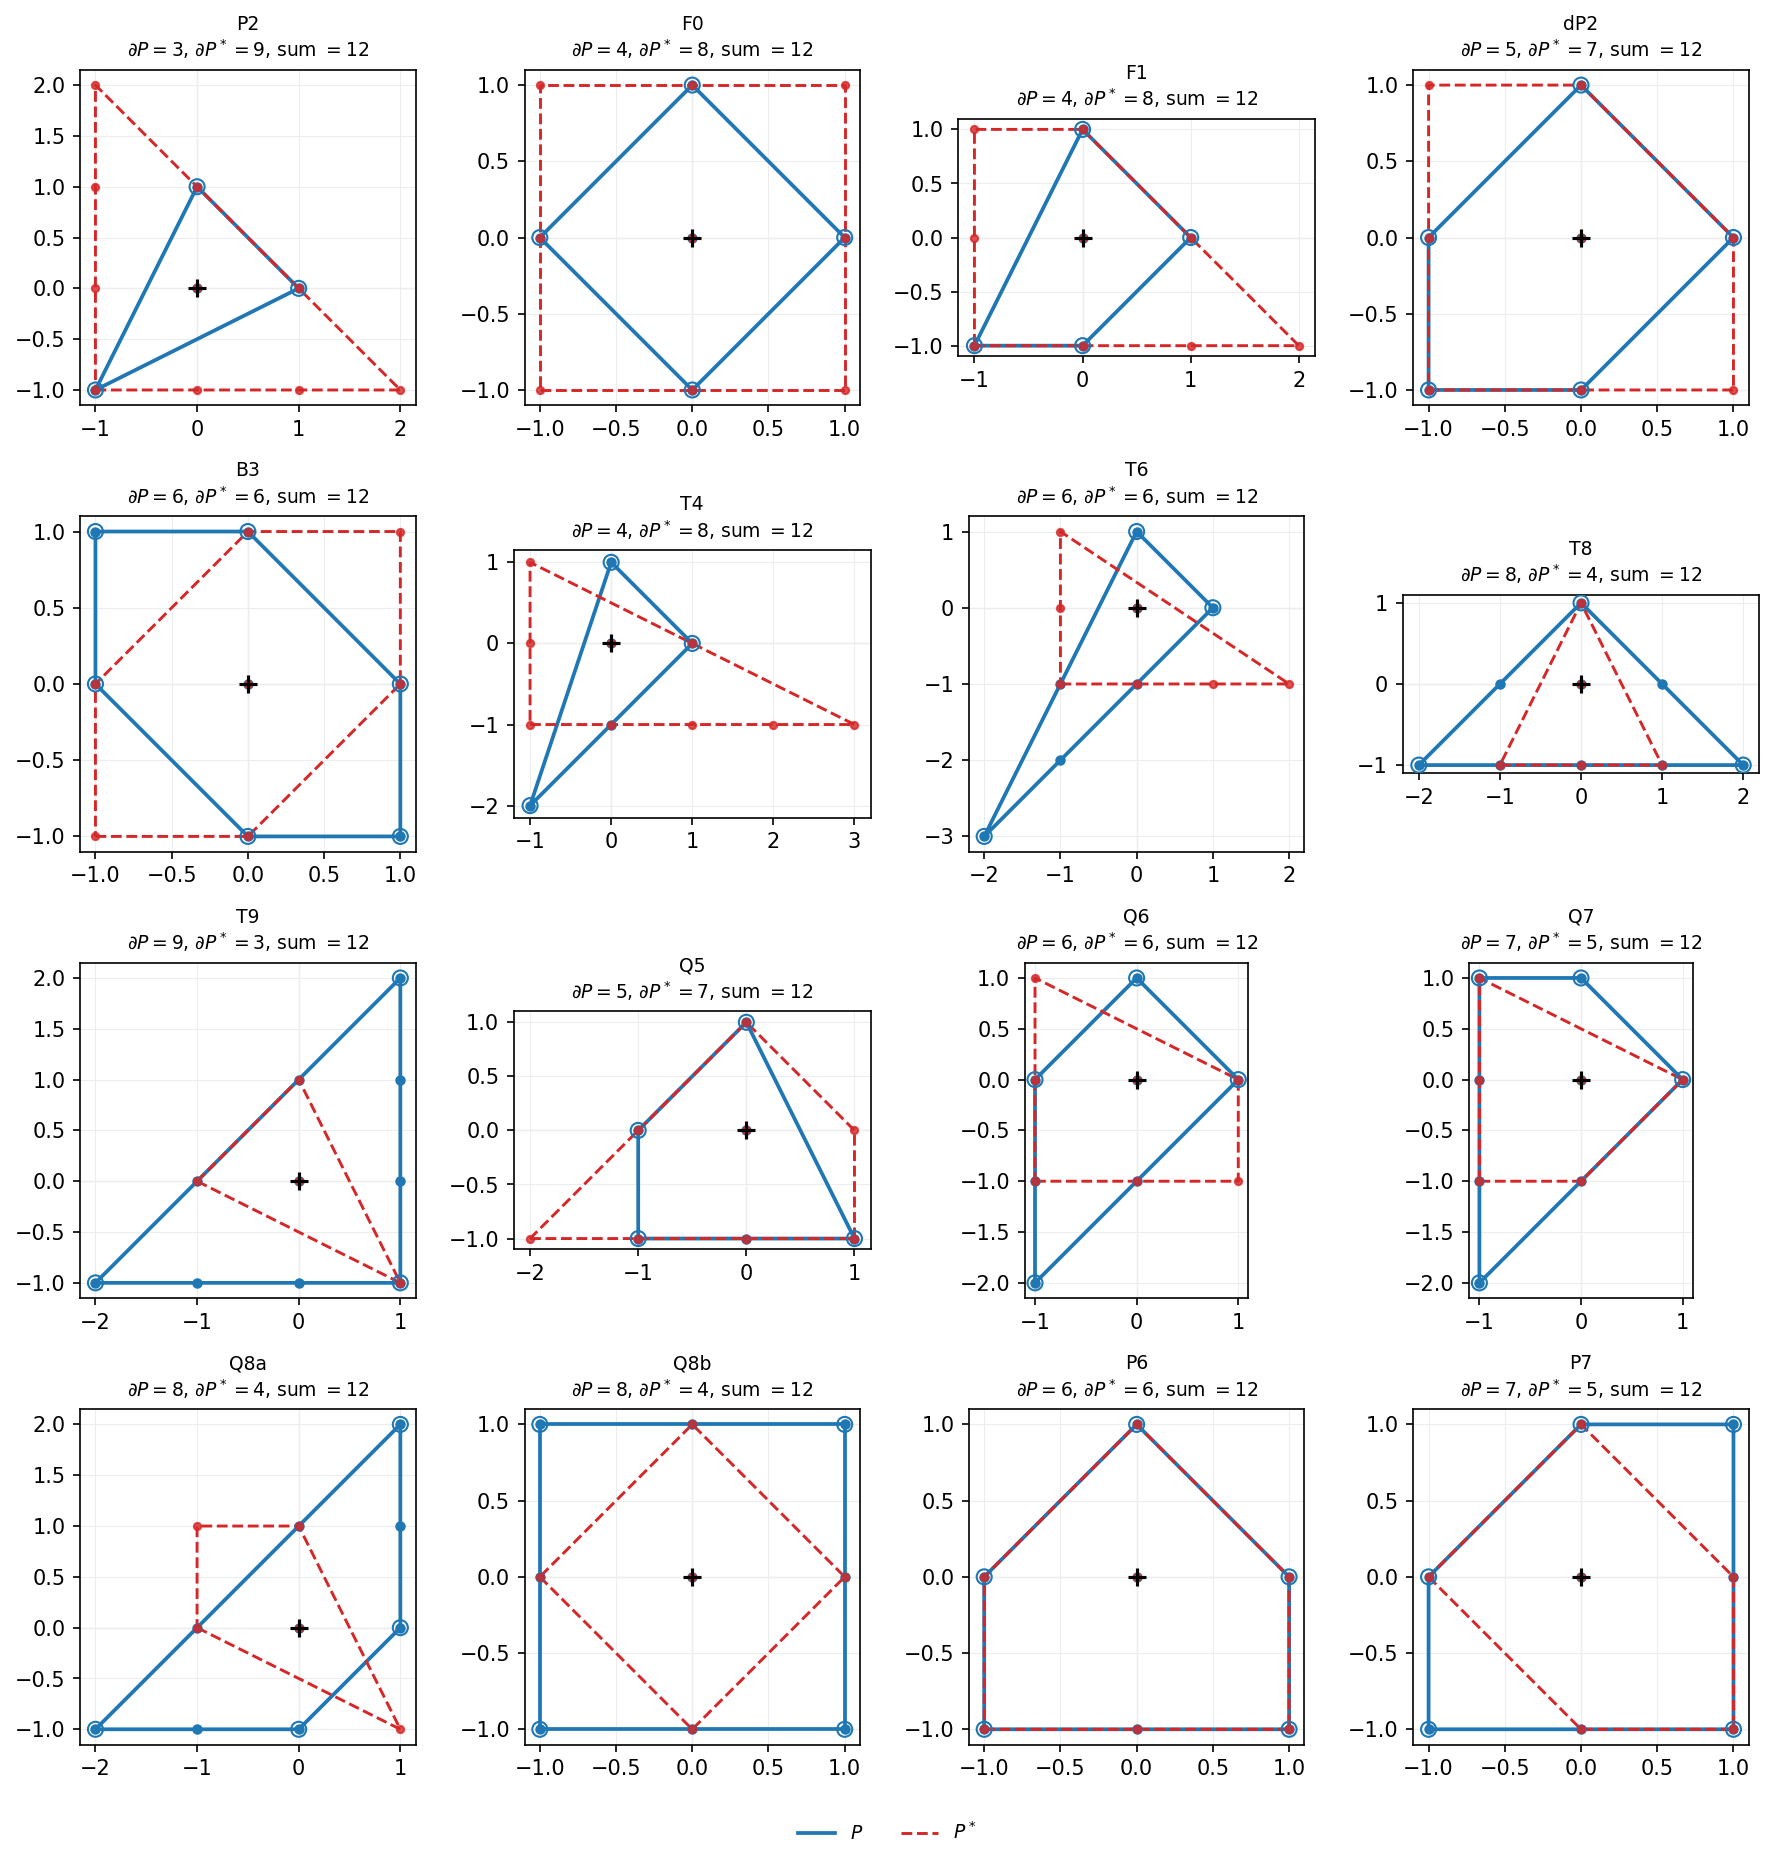
\includegraphics[width=0.7\textwidth]{fig_polygons}
  \caption{\tiny All sixteen two-dimensional reflexive polygons, each drawn with
  its lattice points (solid) and its polar dual $P^{*}$ (dashed). Each polygon
  is the toric diagram of a local \CY{} threefold $K_S$, and the dual is the
  Batyrev mirror. Every title records the twelve theorem,
  $\#\partial P + \#\partial P^{*} = 12$, which holds in all sixteen cases
  however the boundary points are shared out. The classification is not
  assumed by the package: \texttt{toric.verify\_named()} rederives the list by
  brute force, and the five smooth cases --- $\PP^2$, $F_0$, $F_1$, $dP_2$ and
  $B_3 = dP_3$ --- are detected by the criterion that the vertex count equal
  the boundary count, rather than tabulated.}
  \label{fig:polygons}
\end{figure}


%newfig
\FloatBarrier
\section{Knots}


\begin{minipage}[c]{0.4\textwidth}
\small
Figure 4-A - \tiny Upper: the Jones polynomial of $K15n81556$ against that of its
  mirror. Lower: the connected sum $7_1 \# m7_1$ as a braid closure.
\tiny
The upper panel compares the Jones polynomial of the fifteen-crossing census
knot $K15n81556$ with that of its mirror image, coefficient by coefficient.
The two are reflections of one another about $t^0$ and do not coincide, so the
knot is chiral. This reproduces the observation of Wang and
Zhang \cite{WZ2025} that the two diagrams of $K15n81556$ appearing in the
Brittenham--Hermiller argument \cite{BH2025} represent a chiral knot and its
mirror rather than the same knot. The determinant is $39$ for both, so
detecting the chirality requires an invariant that is not symmetric under
$t \mapsto 1/t$.

The lower panel shows the connected sum $7_1 \# m7_1$, whose unknotting number
breaks additivity, drawn as a braid closure. The connected sum of two braid
closures is the juxtaposition of their words on one more strand than the two
together, so this is the closure of $\sigma_1^{7}\sigma_2^{-7}$ on three
strands; the two halves have visibly opposite handedness. The Jones
polynomials are computed by a Kauffman bracket over $2^n$ states in pure
Python, with no external knot-theory dependency.

\end{minipage}
\hfill
\begin{minipage}[c]{0.6\textwidth}
  \centering
  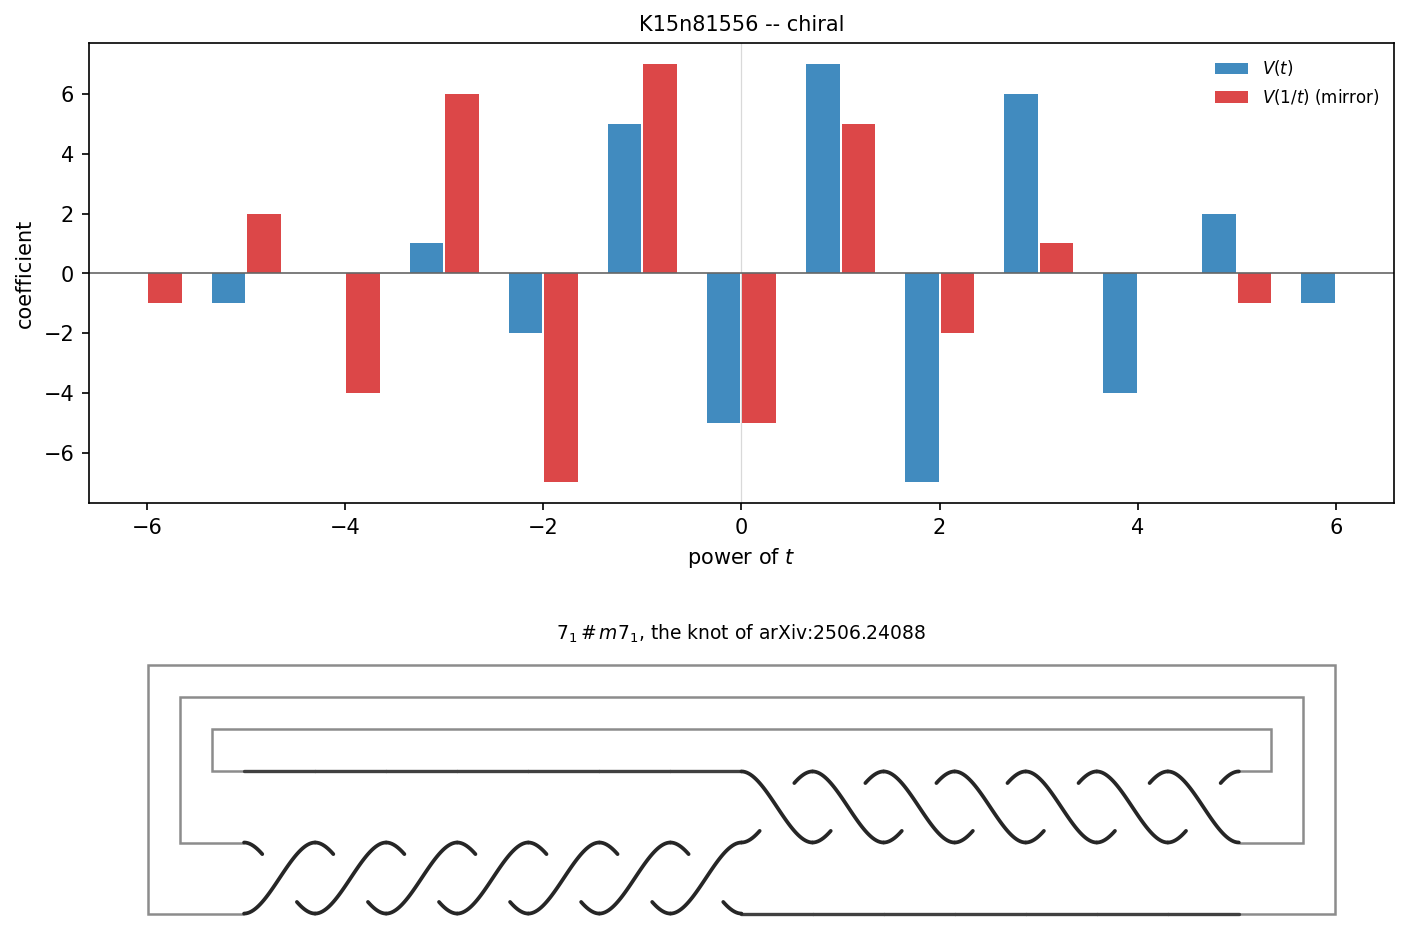
\includegraphics[width=0.9\textwidth]{fig_knots}
  \label{fig:knots}
\end{minipage}


\FloatBarrier
\section{Hofstadter spectra of quantized mirror curves}

\begin{figure}[htbp]
  \centering
  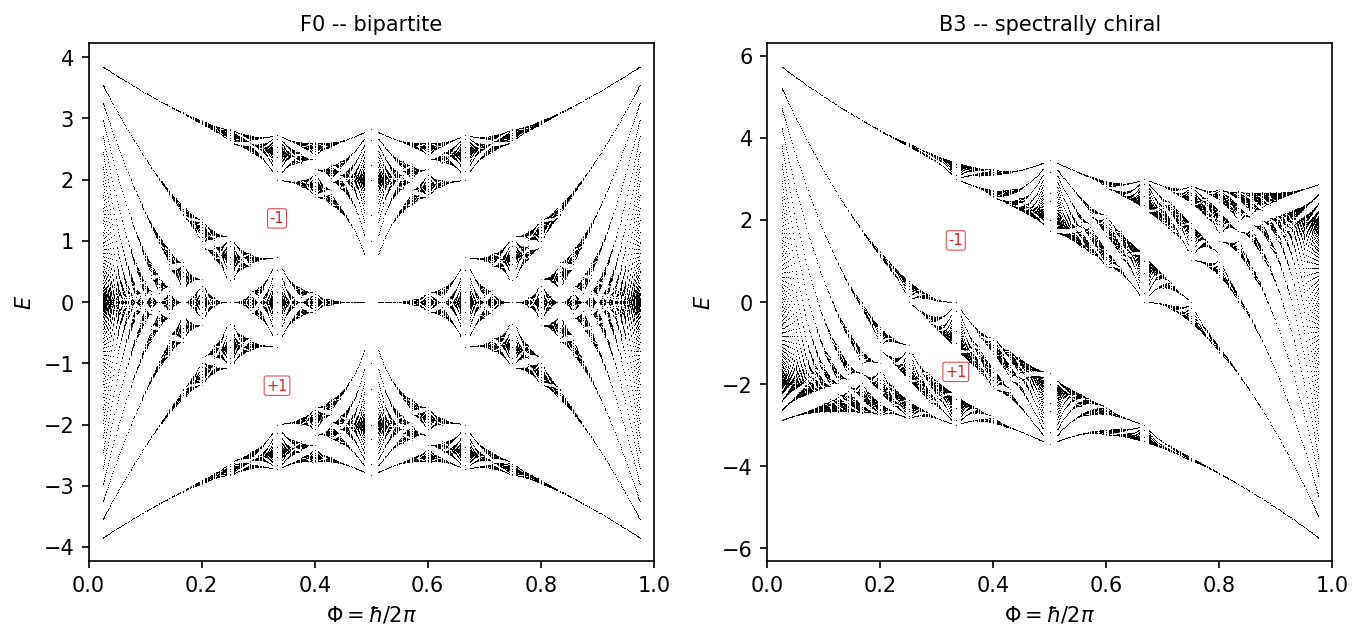
\includegraphics[width=0.95\textwidth]{fig_butterflies.png}
  \caption{\small Hofstadter spectra of the quantized mirror curves of local $F_0$
  (left) and local $B_3 = dP_3$ (right), with gap Chern numbers annotated at
  $\Phi = 1/3$.}
  \label{fig:butterflies}
\end{figure}
\footnotesize
Quantizing the mirror curve of a local toric \CY{} threefold turns it into an
electron hopping on a two-dimensional lattice in a magnetic
field \cite{Sugimoto2017}, under the dictionary: lattice points of the Newton
polygon are hopping vectors, and $\hbar/2\pi$ is the flux per unit cell. The
square polygon of local $F_0$ gives the square lattice and the classic
butterfly; the hexagonal polygon of local $B_3$ gives the triangular lattice.
The gap labels are obtained from the Diophantine equation $r = qs_r + pt_r$
with $|t_r| \le q/2$.

The triangular butterfly is visibly slanted. The reason is that
$E(\Phi) = -E(1-\Phi)$ holds for all sixteen geometries, while
$E(\Phi) = E(1-\Phi)$ holds only in the bipartite cases. Bipartiteness is a
condition on the polygon \emph{modulo two} --- the existence of an
$f \in (\mathbb{Z}/2)^2$ odd on every hopping vector --- and not a reflection
symmetry of it. Only $F_0$ and $T4 = \PP(1,1,2)$ are bipartite, so fourteen of
the sixteen spectra are asymmetric in $E$. Notably $B_3$ is centrally
symmetric as a polygon and still spectrally chiral, while $T4$ is not
centrally symmetric and is spectrally symmetric.


%newfig
\FloatBarrier
\section{Chirality across domains}
\label{sec:chirality}

\begin{figure}[htbp]
  \centering
  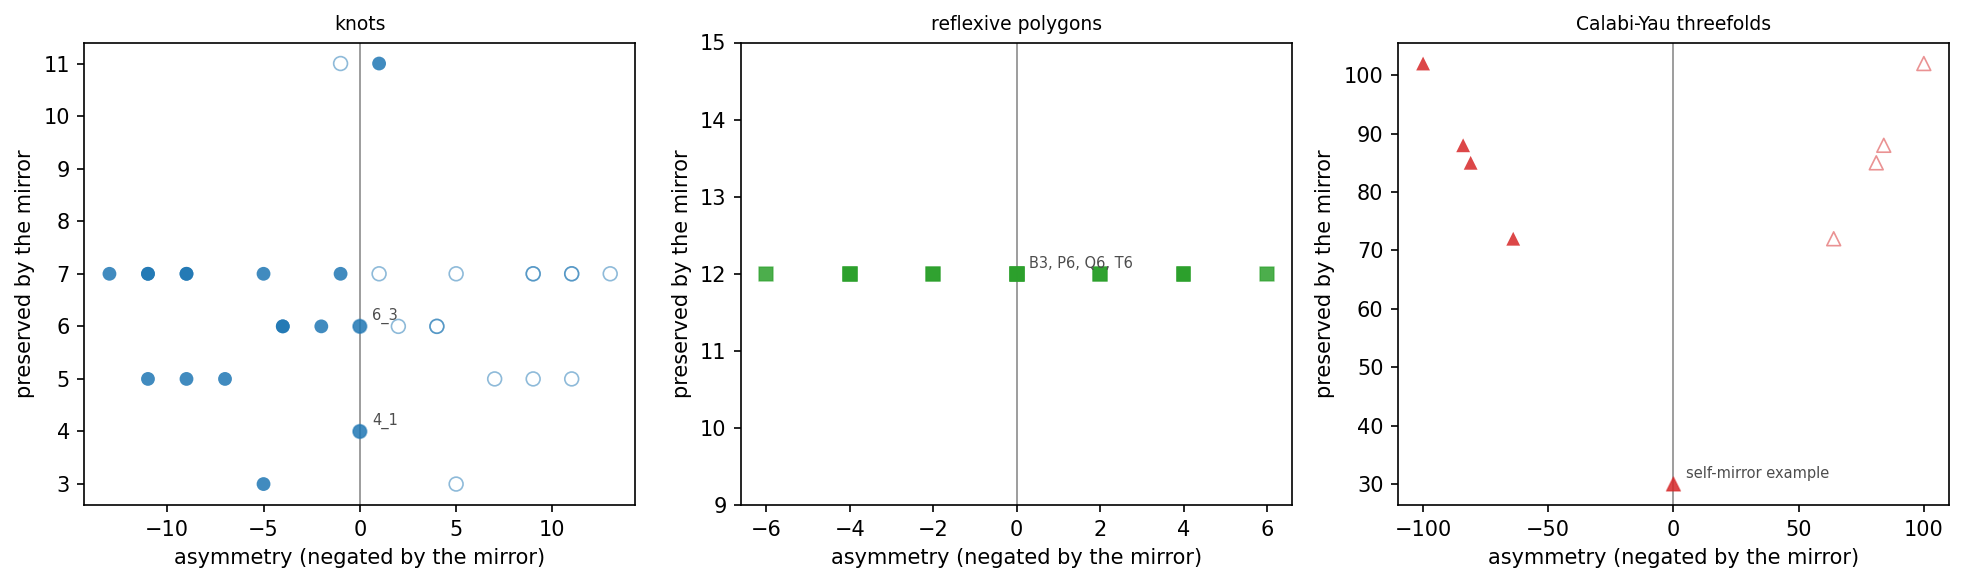
\includegraphics[width=0.9\textwidth]{fig_chirality}
  \caption{ \footnotesize One mirror operation over knots, reflexive polygons and \CY{}
  threefolds. Horizontally the combination the mirror negates, vertically the
  one it preserves; filled markers are the objects, hollow their mirrors.}
  \label{fig:chirality}
\end{figure}
\footnotesize
Three of the mirror operations in this package have the same shape. Each is an
involution that swaps a pair of integers and preserves their sum or span: for
knots the mirror image swaps the extreme degrees of $V(t)$ and preserves the
span; for reflexive polygons polar duality swaps $\#\partial P$ and
$\#\partial P^{*}$ and preserves their sum, which is $12$; for \CY{} threefolds
mirror symmetry swaps $h^{1,1}$ and $h^{2,1}$ and preserves their sum. Mirror
partners therefore sit symmetrically about zero and objects fixed by their
involution lie on the axis. The right-hand panel is the conventional Hodge plot
in disguise, since the horizontal coordinate there is $\chi/2$.

That the preserved quantity is meaningful on the knot side follows from the
Kauffman--Murasugi--Thistlethwaite theorem: the span of $V$ equals the crossing
number exactly for alternating knots, which holds for all fourteen alternating
entries of the built-in table and fails, as it must, for the three
non-alternating ones.

Quantized curves are absent from this figure, and deliberately so. Their
natural involution, reflection of the Newton polygon, leaves the spectrum
\emph{exactly} unchanged, so no spectral invariant can detect it and the
package reports the result as undetermined rather than as achiral. The property
the spectrum does see is bipartiteness, which is logically independent: all
four combinations of the two occur among the sixteen polygons.

Applying the same question to the published list of $7890$ CICY threefolds
gives a sharp answer. Of the $265$ distinct Hodge pairs occurring in it ---
after excluding twenty-two entries that record $0$ for both Hodge numbers, a
sentinel for ``not given'' on the product configurations --- the only pairs
whose mirror also appears are the two self-mirror pairs $(15,15)$ and
$(19,19)$. The list therefore contains no non-trivial mirror pair at all:
$h^{1,1}$ never exceeds $19$ while $h^{2,1}$ reaches $101$, equivalently every
Euler characteristic in the list is non-positive.


\FloatBarrier
\section{A-polynomials and colored Jones}

\begin{minipage}[c]{0.3\textwidth}
Figure 6-A  - \tiny Upper: Newton polygons of the A-polynomials of the figure-eight
  knot and the trefoil, with coefficients and edge slopes annotated. Lower:
  colored Jones polynomials of the trefoil, one row per colour.

The edge slopes shown in the upper panels are boundary slopes of
incompressible surfaces in the knot complement \cite{CCGLS1994}, and they come
out at $\pm 4$ for the figure-eight and $6 = pq$ for the trefoil.

The lower panel shows the colored Jones polynomials $J_N$ of the trefoil,
computed from the Rosso--Jones formula in the form used by Hikami and
Lovejoy \cite{HL2014}, with marker shape giving the sign of the coefficient.
The span grows quadratically in $N$. The row $N = 2$ is the ordinary Jones
polynomial and agrees coefficient for coefficient with the Kauffman-bracket
computation elsewhere in the package --- a representation-theoretic sum over
$2N-1$ terms against a sum over $2^n$ smoothings, from code sharing nothing.

The same lattice points shown above are what the quantized-curve machinery
consumes as a hopping set, which is the concrete link between the two ends of
the package. That link is a statement about the quantization rule and not
about the geometry: the AJ operators satisfy $LQ = qQL$, the same Weyl algebra
used for mirror curves with $q = e^{i\hbar}$, but a toric diagram is a
\emph{reflexive} polygon and an A-polynomial's Newton polygon is not, so the
quantized A-polynomial is not the mirror curve of any local \CY{}.

\end{minipage}
\hfill
\begin{minipage}[c]{0.7\textwidth}
  \centering
  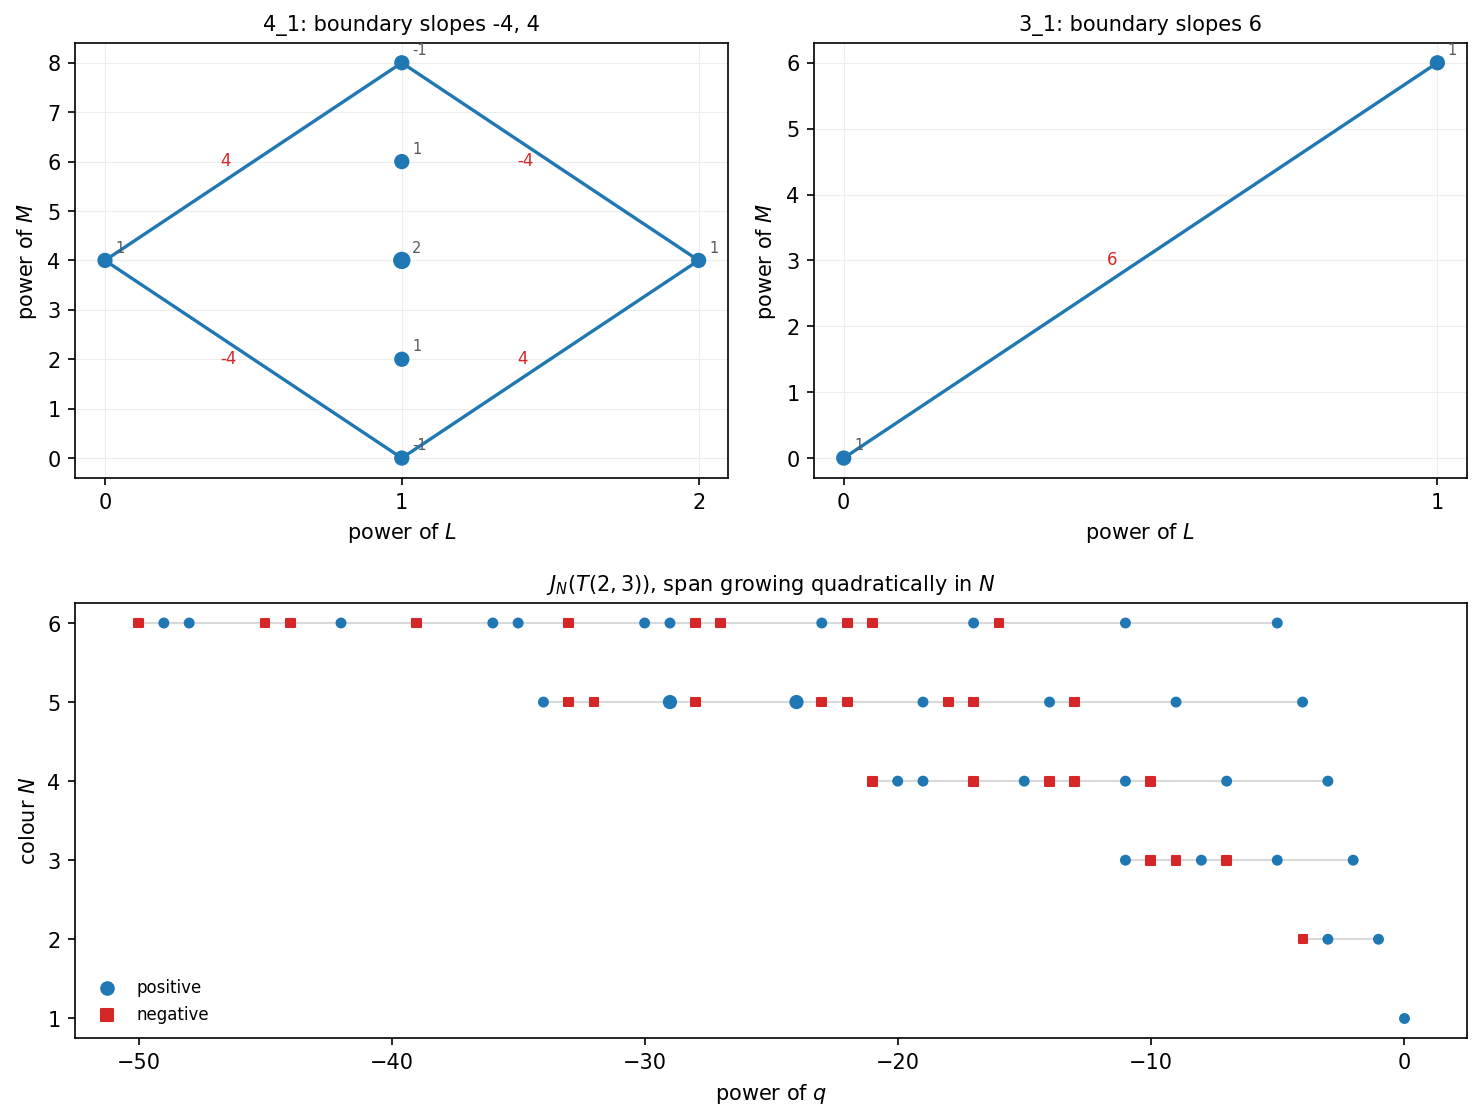
\includegraphics[width=1\textwidth]{fig_apolynomial}
  \label{fig:apolynomial}
\end{minipage}


\FloatBarrier
\section{The quintic cross-section}

\begin{minipage}[c]{0.7\textwidth}
Figure 7:
\newline
The classical Fermat cross-section of the quintic, the degree-five
  hypersurface in $\PP^4$ with configuration $[[4,5]]$, labelled with its
  Hodge numbers. The surface is the projection to three real dimensions of the
  $n^2$ patches of $z_1^n + z_2^n = 1$, evaluated directly in complex
  arithmetic.
\end{minipage}
\hfill
\begin{minipage}[c]{0.3\textwidth}
\centering
  \includegraphics[width=0.9\textwidth]{quintic_surface.png}
  \label{fig:quintic}
\end{minipage}




\FloatBarrier
\section{Hyperbolic lattices}

\begin{minipage}[c]{0.4\textwidth}
Figure 8: 
\newline 
\tiny
Left: a patch of the $\{8,8\}$ tessellation in the Poincar\'e disk,
  with bonds drawn as true geodesics and colour recording the ring index.
  Right: the boundary fraction against flake depth, with the limit
  $(p-2)/(p-1)$ dashed.

The marked points in the left panel are cell centres, which for the
$\{4g,4g\}$ family form the Bravais lattice of a genus-$g$ surface. Bonds are
circular arcs meeting the disk boundary at right angles, not chords.

The right panel measures the fraction of cells that are not fully coordinated.
It does not tend to zero. Each ring is larger than the last by a factor $p-1$,
so the fraction on the rim tends to $(p-2)/(p-1)$, which is $6/7$ for
$\{8,8\}$ and $10/11$ for $\{12,12\}$; the measured points approach that limit
from above. A finite patch is therefore never a good approximation to the bulk,
which is the quantitative reason hyperbolic band theory requires periodic
boundary conditions and automorphic functions \cite{MR2022} rather than a
large-flake extrapolation.
\end{minipage}
\begin{minipage}[c]{0.55\textwidth}
  \centering
  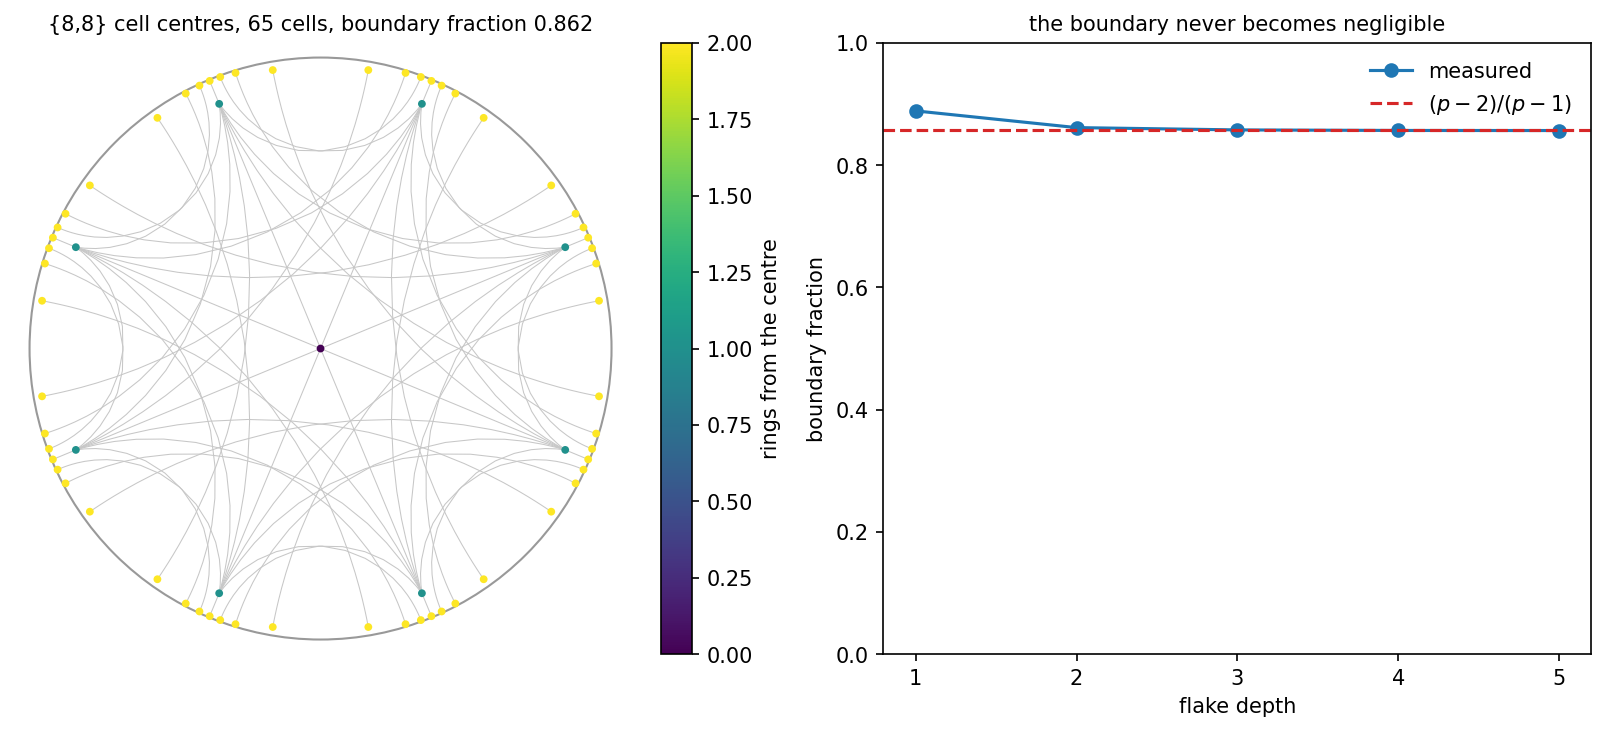
\includegraphics[width=0.9\textwidth]{fig_hyperbolic}
  \label{fig:hyperbolic}
\end{minipage}

\footnotesize

For the $\{4g,4g\}$ tessellations the package constructs the $4g$ side-pairing
translations, verifies that they pair into inverses and satisfy the relator
$\gamma_0\gamma_1^{-1}\gamma_2\gamma_3^{-1}\cdots = 1$ of the regular
$4g$-gon with opposite sides identified, and confirms the genus independently
by Gauss--Bonnet, the cell area being exactly $4\pi(g-1) = 2\pi|\chi|$. It is
worth noting that this relator is \emph{not} the canonical surface word
$\prod_i [a_i,b_i] = 1$: the two present the same group in different
generators, and the canonical word evaluated on these generators is nowhere
near the identity.



\FloatBarrier
\section{Node counts along split edges}

\begin{minipage}[c]{0.4\textwidth}
Figure 9:
\newline
Distribution of the node count $N$ over the edges of the web. Each
  edge is a conifold transition, and $N$ is the number of nodes acquired at
  the singular point of the transition.
\end{minipage}
\hfill
\begin{minipage}[c]{0.55\textwidth}
\centering
  \includegraphics[width=0.8\textwidth]{node_counts}
  \label{fig:nodes}
\end{minipage}


\FloatBarrier
\section{Gopakumar--Vafa invariants}
\begin{minipage}[c]{0.4\textwidth}
Figure 10:
\newline
Genus-zero Gopakumar--Vafa invariants of the five one-parameter
  complete intersection models, plotted on a logarithmic scale against the
  degree. The quintic entries reproduce the classical values
  $2875$, $609250$, $317206375$, which serve as a check on the enumerative
  machinery rather than as new output.
\end{minipage}
\hfill
\begin{minipage}[c]{0.5\textwidth}
\centering
  \includegraphics[width=0.8\textwidth]{gv_invariants}
  \label{fig:gv}
\end{minipage}


\FloatBarrier
\section{Growth of the web}
\begin{minipage}[c]{0.5\textwidth}
Figure 11:
\newline
Growth of the web with splitting depth, counted both in
  configurations reached and in distinct Hodge pairs realised. The number of
  configurations grows far faster than the number of distinct topological
  types, which is the reason the normal form of
  \pkg{pyCICY.transitions} is needed: without it, relabellings would be
  counted as new manifolds.
\end{minipage}
\hfill
\begin{minipage}[c]{0.5\textwidth}
\centering
  \includegraphics[width=0.9\textwidth]{web_growth}
  \label{fig:growth}
\end{minipage}


\section{Scope and limitations}

Several things in this supplement are quoted rather than derived, and the
distinction is maintained in the code as well as here.

\begin{itemize}
  \item Unknotting numbers are minima over all diagrams and are not
  accessible from a single diagram; they are quoted from the literature. The
  crossing-change search provided by the package gives diagram-dependent
  upper bounds only, and does not recover the Brittenham--Hermiller bound by
  brute force --- which is the point, since the economical route is not
  visible in the obvious diagram.
  \item A-polynomials are quoted with attribution. Deriving one means
  eliminating variables from the gluing equations of a triangulation, which
  is a separate undertaking.
  \item The recursion search underlying the AJ verification returns the
  smallest $L$-degree admitting a solution \emph{within the chosen search
  bounds}; widening or narrowing the bounds moves the answer, and no claim of
  minimality is made. The classical limit of an annihilating operator contains
  the A-polynomial as a factor but need not equal it, and the extra factor is
  reported rather than divided away.
  \item For hyperbolic lattices, the enumeration of normal subgroups of a
  Fuchsian group is not implemented; that is what would give the complete set
  of irreducible representations and hence the full spectrum, and it is a
  computational group theory problem better handed to a dedicated system. The
  representation sectors computed here are genuine sectors but are not
  claimed to exhaust anything.
  \item source code: \url{https://github.com/brentharts/CICY}

\end{itemize}


\begin{thebibliography}{9}

\bibitem{Anderson2025}
L.~B.~Anderson, J.~Gray, S.~A.~Patil and C.~Scanlon,
\emph{Mapping moduli across heterotic conifolds},
\href{https://arxiv.org/abs/2512.18124}{arXiv:2512.18124}.


\bibitem{BH2025} M.~Brittenham and S.~Hermiller,
\emph{Unknotting number is not additive under connected sum},
arXiv:2506.24088.

\bibitem{WZ2025} C.~Wang and Y.~Zhang,
\emph{A remark on the counterexample to the unknotting number conjecture},
arXiv:2507.14265.

\bibitem{Sugimoto2017} Y.~Sugimoto,
\emph{Calabi--Yau geometry and electrons on 2d lattices},
Phys.\ Rev.\ D \textbf{95} (2017) 086004, arXiv:1701.01561.

\bibitem{MR2022} J.~Maciejko and S.~Rayan,
\emph{Automorphic Bloch theorems for hyperbolic lattices},
Proc.\ Natl.\ Acad.\ Sci.\ USA \textbf{119} (2022) e2116869119.

\bibitem{CCGLS1994} D.~Cooper, M.~Culler, H.~Gillet, D.~D.~Long and
P.~B.~Shalen, \emph{Plane curves associated to character varieties of
3-manifolds}, Invent.\ Math.\ \textbf{118} (1994) 47.

\bibitem{HL2014} K.~Hikami and J.~Lovejoy,
\emph{Torus knots and quantum modular forms},
arXiv:1409.6243.

\bibitem{CDLS1988} P.~Candelas, A.~M.~Dale, C.~A.~L\"utken and
R.~Schimmrigk, \emph{Complete intersection Calabi--Yau manifolds},
Nucl.\ Phys.\ B \textbf{298} (1988) 493.



\end{thebibliography}

\end{document}
